\chapter{MEV and Fair Transaction Ordering}

\section{Front running}
Front running is the act of placing a transaction in a queue with the knowledge of a future transaction. Front running on a blockchain platform normally happens when a miner, who has access to information on pending transactions, places an order that would earn him a profit based on a pending trade.\\\\
For example, if a broker knows that a large client is about to buy a lot of shares of a certain company, they may buy some shares for themselves first and then sell them at a higher price after the client’s order is executed. This way, they can profit from the price increase caused by the client’s order.
\begin{figure}[h!]
	\centering
	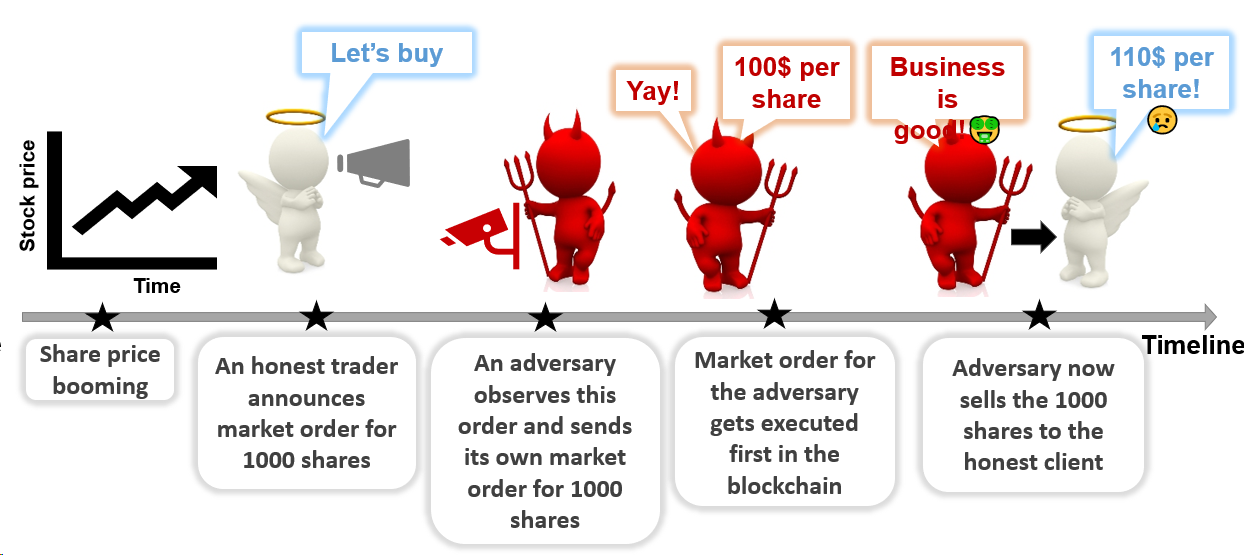
\includegraphics[width=0.7\linewidth]{Fig/21/F1}
	\caption{An example of front running}
	\label{fig:L21_f1}
\end{figure}\\	
Front running is illegal and unethical, as it violates the duty of loyalty and confidentiality that brokers owe to their clients. It also harms the market efficiency and fairness, as it creates artificial price movements and disadvantages other investors who do not have access to the same information

\subsection{HFT}
High-frequency trading (HFT) is a form of trading that uses advanced algorithms and technology to execute orders at extremely high speeds, often in fractions of a second. HFT firms use their speed advantage to exploit inefficiencies and loopholes in the market, such as front-running, arbitrage, and market manipulation. 

\subsection{Front running in Defi}
In DeFi, front-running strategies exploit both public knowledge of user trades from transactions pending on the network and the miner’s ability to determine the final transaction order. Given the financial loss and increased transaction load resulting from adversarial front-running in decentralized finance, novel cryptographic protocols have been proposed to mitigate such attacks in the permission-less blockchain setting. Some of these protocols include fair ordering, batching of blinded inputs, commit and reveal schemes, private user balances, secret input stores, and zero-knowledge proofs.

\subsection{Miner’s incentives}
Miners in a blockchain network can choose to order transactions based on their fees, rather than their arrival time. This is a form of front-running. Figure \ref{fig:L21_f2} shows an example of three transactions that arrive at different times, but have different fees attached to them. A rational miner would prefer to order the transactions based on their fees, rather than their arrival time, as this would maximize their profit. Therefore, the miner would put $tx_1$ and $tx_3$ before $tx_2$, even though $tx_2$ arrived earlier. Ordering by first-in-first-out (FIFO) is a myth, as miners have the power and incentive to manipulate the order of transactions in a block.
\begin{figure}[h!]
	\centering
	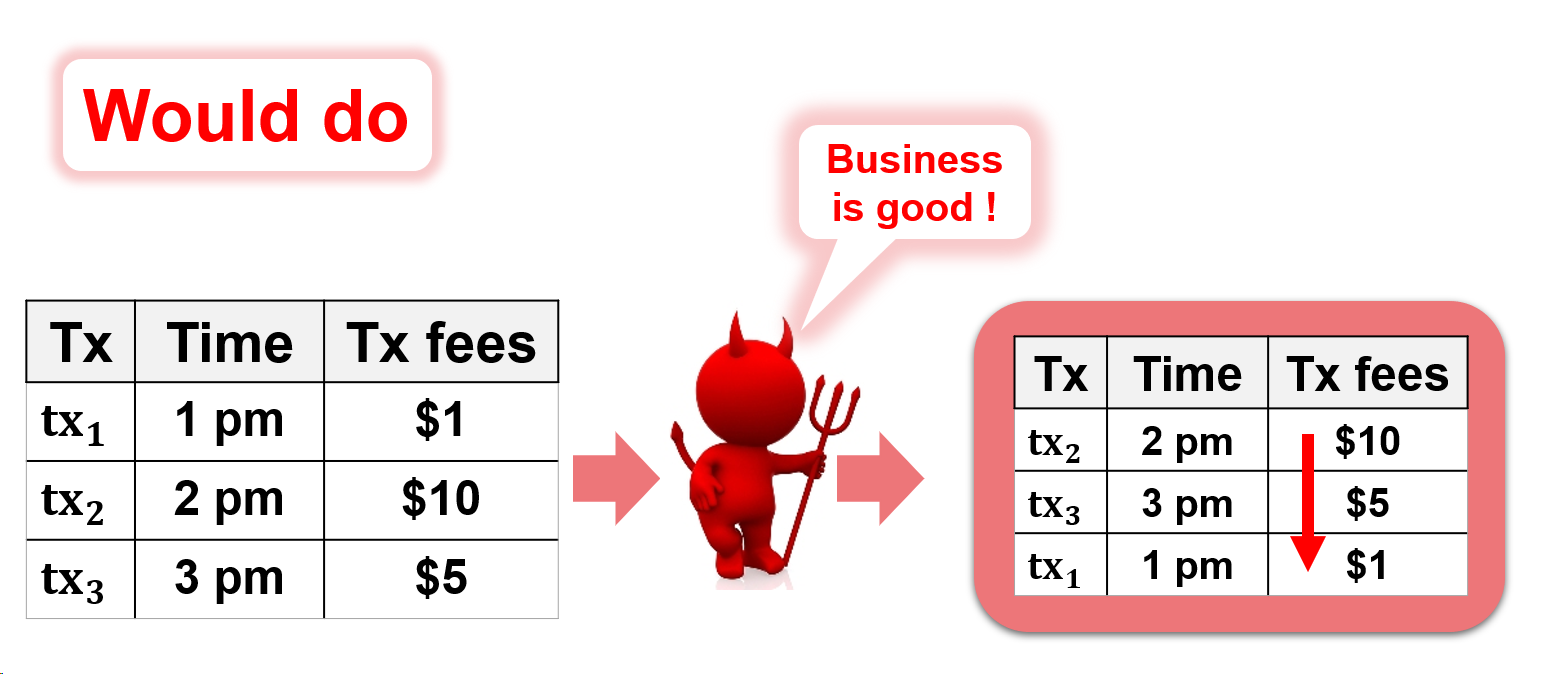
\includegraphics[width=0.5\linewidth]{Fig/21/F2}
	\caption{Ordering transactions based on their fees, rather than their arrival time}
	\label{fig:L21_f2}
\end{figure}

\subsection{DEX}
A decentralized exchange (DEX) is a type of cryptocurrency exchange that allows users to trade digital assets without relying on a centralized intermediary, such as a broker, bank, or custodian. A DEX operates on a peer-to-peer (P2P) network, where users can directly interact with each other and execute transactions through smart contracts. A DEX aims to provide more security, privacy, transparency, and control to the users, as they do not have to trust or depend on a third party to manage their funds or data.\\\\
The order book is a list of buy and sell orders that are placed by the users on the DEX. The order book also records the transaction history and the current market price of the assets. The order of the transactions matters, as it can affect the price and availability of the assets. For example, if a buyer places an order for 1 BTC at \$50,000 before another buyer places an order for 1 BTC at \$49,000, the first buyer will get their order filled first, while the second buyer may have to wait or pay more. This is also where front-running can occur. For example, if an adversary observes an order for 1 BTC at \$50,000 and submits their own order for 1 BTC at \$50,001 with a higher fee, they can get their order executed first and then sell the BTC to the original buyer at \$50,000, making a profit at their expense.

\section{Miner extractable value (MEV)}
MEV is a measure of the profit that miners or validators can make by manipulating the order, inclusion, or exclusion of transactions in a block. MEV can be exploited by various actors, such as miners, validators, arbitrageurs, liquidators, or bots, who use their speed, power, or knowledge advantage to gain an edge over other users. MEV can create negative effects for the network, such as congestion, instability, unfairness, and reduced trust.\\\\
FIgure \ref{fig:L21_f3} MEV has increased significantly over time, reaching a total of more than \$670 million as of today. (Also see figure \ref{fig:L21_f4} and \ref{fig:L21_f5})
\begin{figure}[h!]
	\centering
	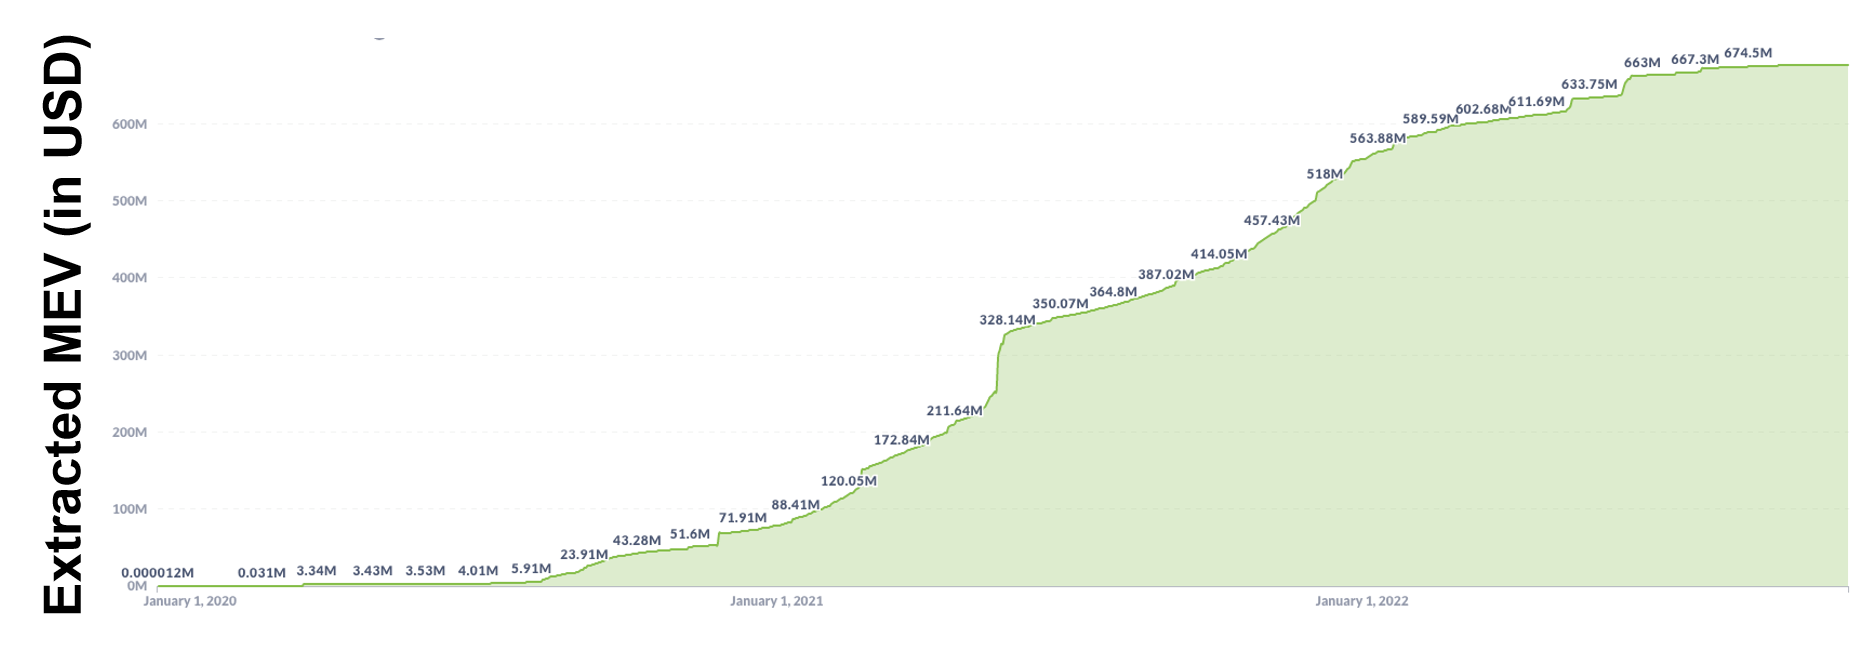
\includegraphics[width=\linewidth]{Fig/21/F3}
	\caption{MEV}
	\label{fig:L21_f3}
\end{figure}
\begin{figure}[h!]
	\centering
	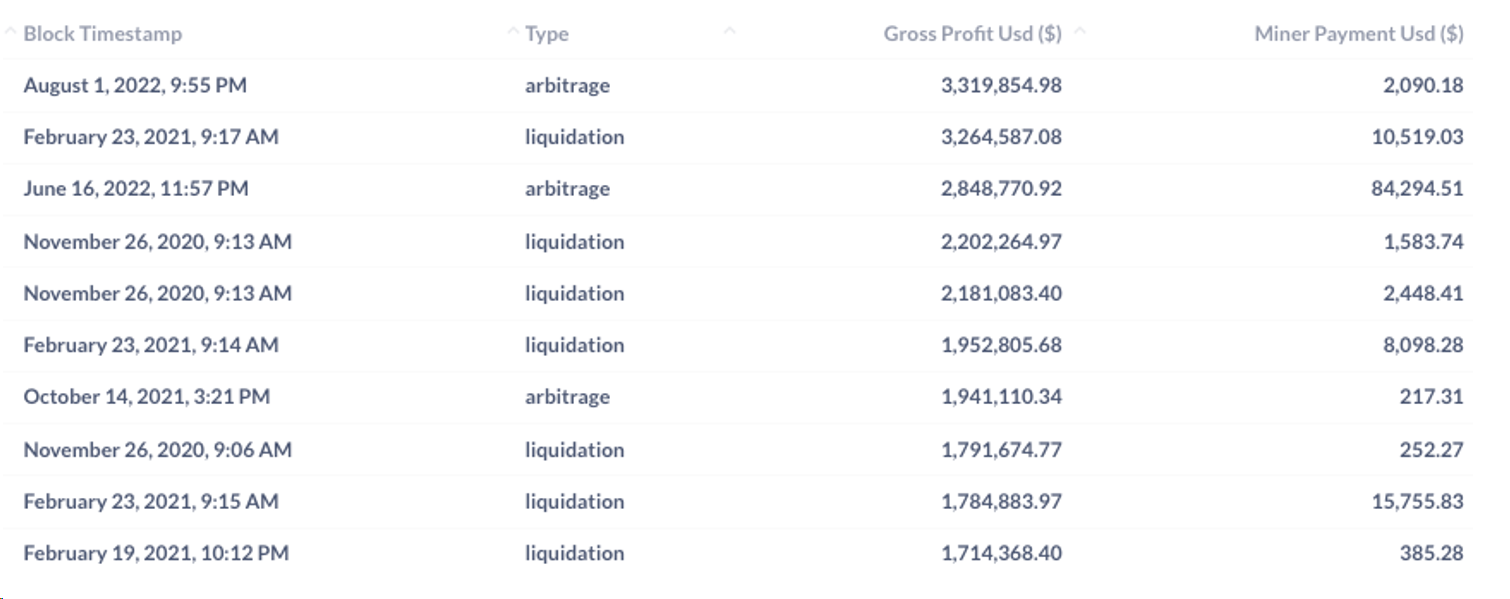
\includegraphics[width=\linewidth]{Fig/21/F4}
	\caption{MEV}
	\label{fig:L21_f4}
\end{figure}
\begin{figure}[h!]
	\centering
	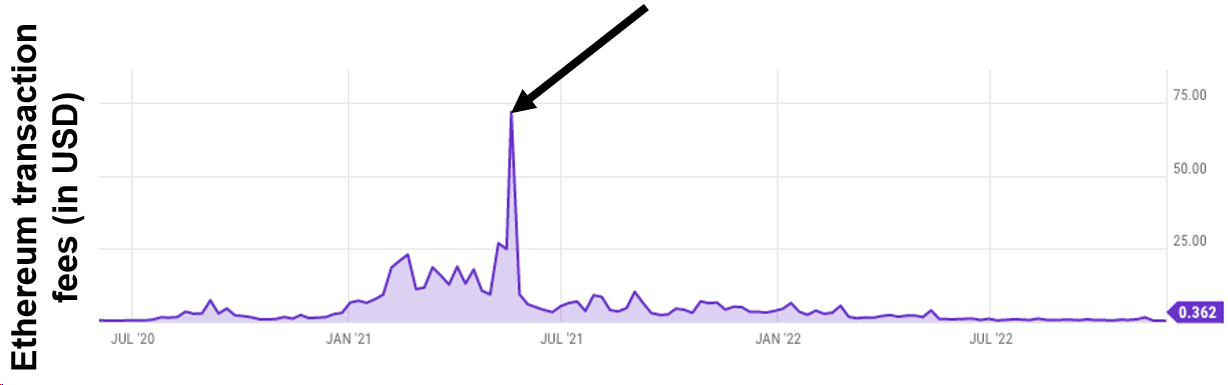
\includegraphics[width=\linewidth]{Fig/21/F5}
	\caption{Ethereum transaction fees}
	\label{fig:L21_f5}
\end{figure}

\section{In search of solutions}
\subsection{EIP 1559}
A solution to front running is EIP-1559, which is a proposal to change the fee market structure of Ethereum. EIP stands for Ethereum Improvement Proposal, which is a document that describes a new feature or improvement for the Ethereum network. EIP-1559 aims to introduce a base fee that is burned and a tip that is paid to miners, creating a more predictable and efficient fee system for users and miners.\\\\
EIP-1559 works by introducing two components to the fee system:
\begin{itemize}
	\item \textbf{Base fee} : the minimum fee that a transaction needs to pay to be included in a block.
	\item \textbf{Tip} : the amount that a user can optionally pay to the miner or validator who includes their transaction in a block.
\end{itemize} 
The base fee is adjusted by the protocol based on the level of network congestion: the fee increases when the network is at greater capacity, and decreases when the network is at lower capacity. The base fee is burned, meaning that it is removed from circulation and reduces the total supply of ETH. This creates a deflationary pressure on ETH and reduces its environmental impact.\\\\
The tip is used to incentivize miners or validators to process transactions faster or to prioritize certain transactions over others. The tip is not burned, but goes to the miner or validator as a reward.\\\\
The miner has two options:
\begin{itemize}
	\item to include the transactions in the order they arrived. In this case, miners will receive a fair tip and avoid wasting gas.
	\item to manipulate the order to extract more value from them. In this case, miners will not gain any profit, as the base fee will be burned and the tip will be negligible.
\end{itemize}
\begin{figure}[h!]
	\centering
	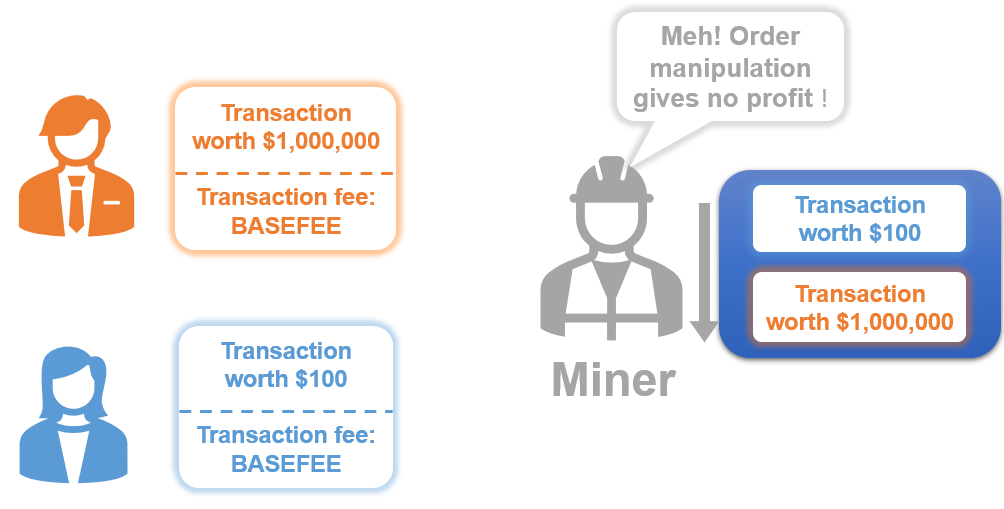
\includegraphics[width=0.6\linewidth]{Fig/21/F6}
	\caption{EIP 1559}
	\label{fig:L21_f6}
\end{figure}

\subsection{Off-chain auction}
An off-chain auction is a way of conducting an auction for a digital asset without using the blockchain to record the bids and the final sale. Instead, the auction is done through a third-party platform or service that handles the communication and verification of the bids, and transfers the ownership of the asset to the highest bidder. Off-chain auctions have some advantages over on-chain auctions, such as lower fees, faster execution, and more privacy. However, they also have some drawbacks, such as relying on a trusted intermediary, being vulnerable to network failures or attacks, and lacking transparency and auditability.
\begin{figure}[h!]
	\centering
	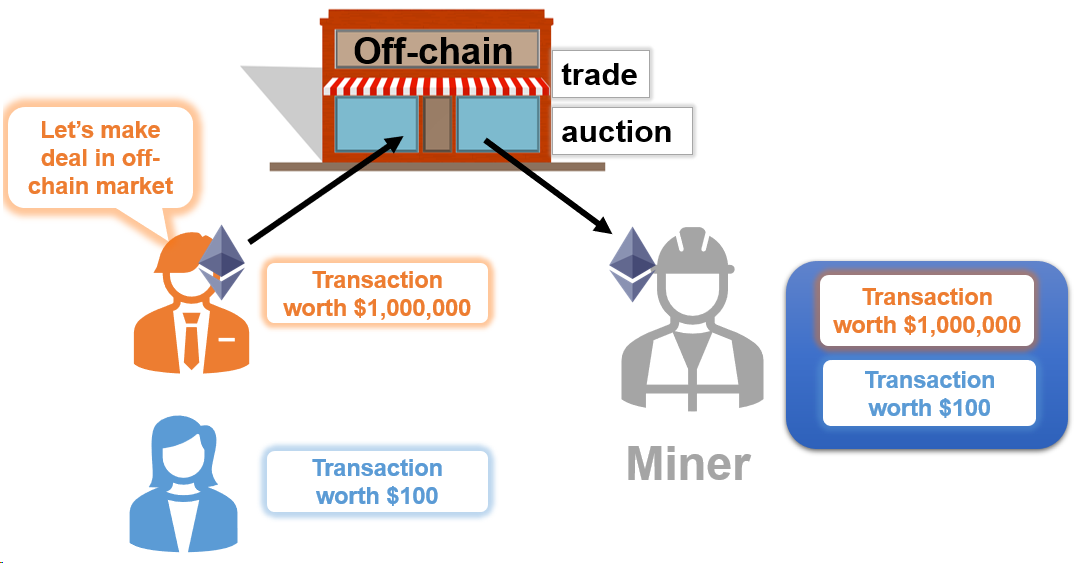
\includegraphics[width=0.6\linewidth]{Fig/21/F7}
	\caption{Off-chain trading}
	\label{fig:L21_f7}
\end{figure}

\section{Order-fairness}
Order-fairness is an important property for blockchain systems, especially for applications that involve financial transactions or smart contracts. Order-fairness means that the order of transactions in the blockchain reflects the order of their submission by the users, without any manipulation or bias by the miners or other parties. Order-fairness can prevent frontrunning attacks.\\\\
However, achieving order-fairness in blockchain systems is challenging, due to the distributed and decentralized nature of the network. Different nodes may have different views of the pending transactions, depending on their network latency and connectivity. Moreover, miners have the incentive to maximize their revenue by selecting transactions with higher fees, regardless of their submission order. Therefore, there is a need for mechanisms that can enforce order-fairness in blockchain systems, either by design or by verification.
\subsection*{Linearizability}
Order-fairness is related to linearizability, which is a stronger form of consistency that guarantees that every operation appears to take effect atomically at some point between its invocation and response. Linearizability is another property that ensures that transactions in a blockchain are ordered in a consistent way, meaning that they appear to be executed atomically and in the same order by all nodes. Linearizability implies order-fairness, but not vice versa. Order-fairness only requires that transactions are ordered according to their submission order, not according to their execution order. Therefore, order-fairness allows for more concurrency and scalability than linearizability. 
\subsection*{Median Fairness}
One definition of order-fairness is median fairness, which requires that the order of transactions in a block is close to the median order of transactions observed by all nodes. This means that the block proposer cannot deviate too much from the average order of transactions seen by the network, and thus cannot favor some transactions over others. However, this definition does not provide any protection from even one Byzantine miner, who can manipulate the order of transactions to their benefit.\\\\
Median fairness is also not very efficient, because it requires all nodes to communicate their observed order of transactions to each other, and then compute the median order. This can be costly and time-consuming, especially in large networks with many transactions. 

\subsection*{$\gamma$-receive-order-fairness}
Another definition of order-fairness is $\gamma$-fraction order-fairness, which requires that the order of transactions in a block conforms with the ordering of most parties. This means that the block proposer cannot deviate too much from the order of transactions observed by at least y-fraction of the nodes, and thus cannot favor some transactions over others. However, this definition assumes that there are no Byzantine nodes, who can act maliciously and disrupt the consensus protocol. If there are Byzantine nodes, they can collude with the block proposer and manipulate the order of transactions to their benefit. Therefore, y-fraction order-fairness is not a secure definition of order-fairness for blockchain systems.\\\\
One way to achieve order-fairness is to prevent any single miner from determining the order of transactions unilaterally. This can be done by collecting the transactions from many miners and then aggregating them according to some criteria. However, achieving order-fairness in this way also poses some challenges, such as how to collect and aggregate the transactions efficiently and securely, and how to deal with conflicting or malicious transactions.

\section{Single Chain Protocol}
One approach to achieve order-fairness is to use a single chain protocol, where all nodes agree on a single sequence of transactions that is consistent and fair. A single chain protocol consists of three steps:
\begin{itemize}
	\item \textbf{Proof-of-work} : a node mines a block by solving a cryptographic puzzle.
	\item \textbf{Semantic chains} : a node confirms the transactions in the block by streaming them to other nodes.
	\item \textbf{Finalization} : a node reaches consensus on the fair ordered ledger by applying some rules. Finalization ensures that the blocks in the chain are consistent and immutable.
\end{itemize} 
\begin{figure}[h!]
	\centering
	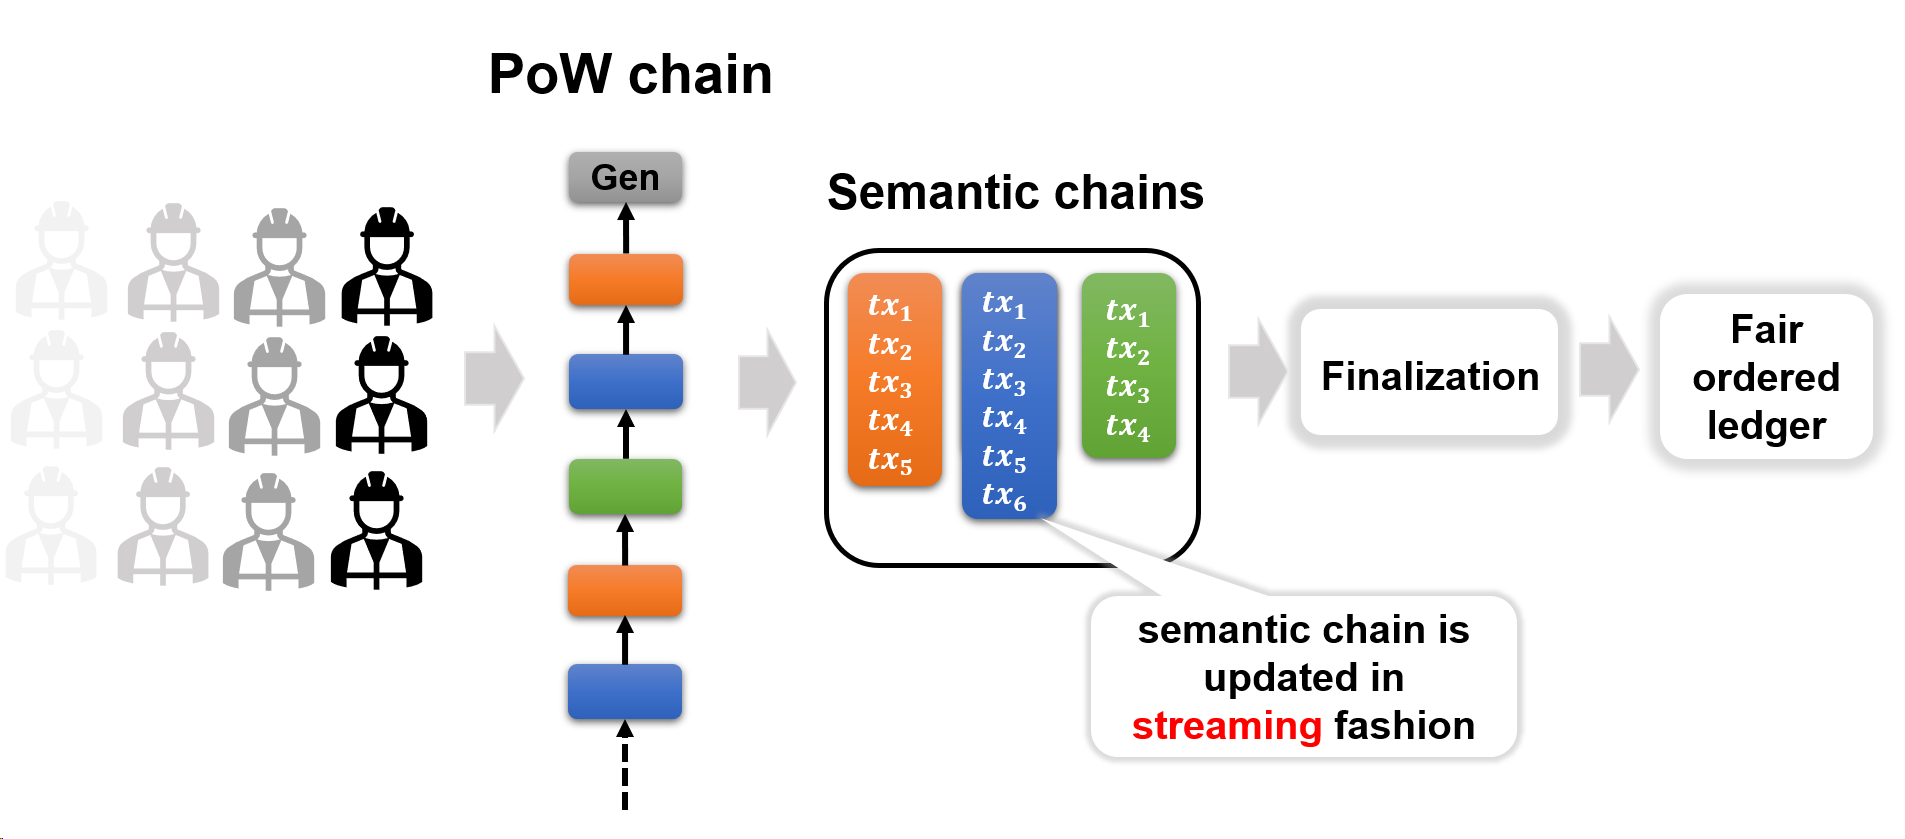
\includegraphics[width=0.7\linewidth]{Fig/21/F8}
	\caption{Single Chain Protocol}
	\label{fig:L21_f8}
\end{figure}
\subsection{Aequitas}
One way to achieve finalization is to use a protocol called Aequitas, which is a single chain protocol that provides order-fairness and Byzantine fault tolerance. \\\\
In the finalization step, each node constructs a dependency graph G, where each node represents a transaction and each edge represents a dependency between transactions. A dependency means that one transaction must appear before another transaction in the fair-ordered ledger. A node can determine the dependencies by looking at the semantic chains, which are streams of transactions confirmed by other nodes. The node then proposes this order to other nodes and reaches consensus on the fair-ordered ledger.\\\\
Aequitas guarantees that the finalization step produces a fair and consistent order of transactions in the blockchain.
\begin{figure}[h!]
	\centering
	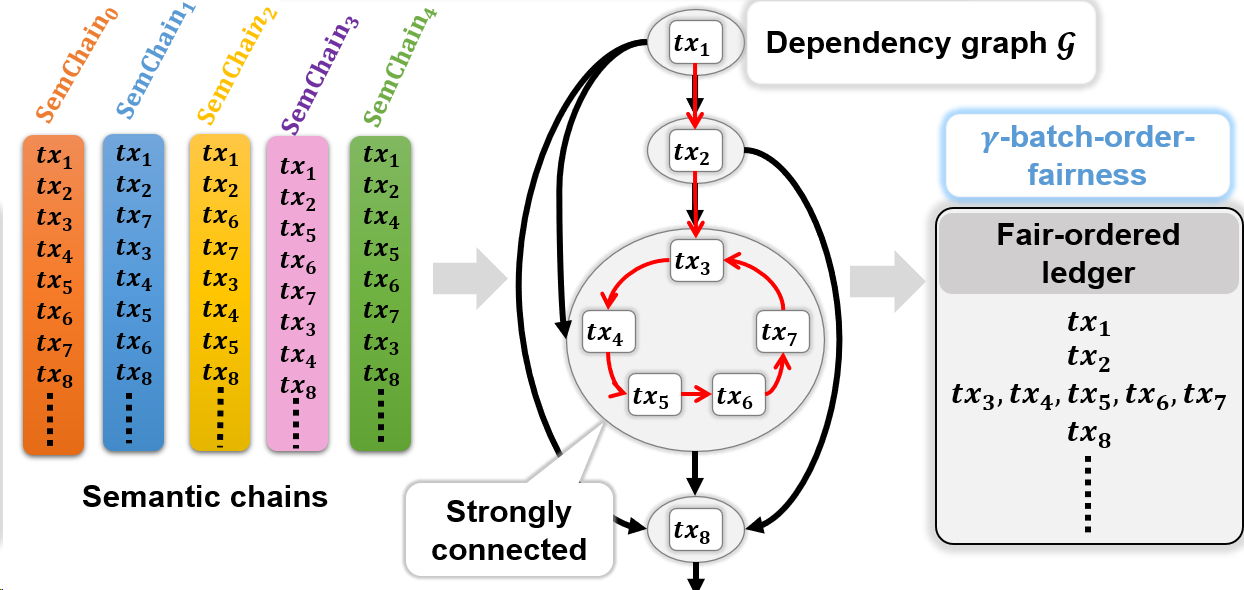
\includegraphics[width=0.7\linewidth]{Fig/21/F9}
	\caption{Aequitas}
	\label{fig:L21_f9}
\end{figure}

\section{Combating latency}
\subsection{Multi-chain}
A multi-chain system is a type of blockchain system that uses multiple chains of blocks to store and validate transactions. A multi-chain system aims to combat latency.
\begin{figure}[h!]
	\centering
	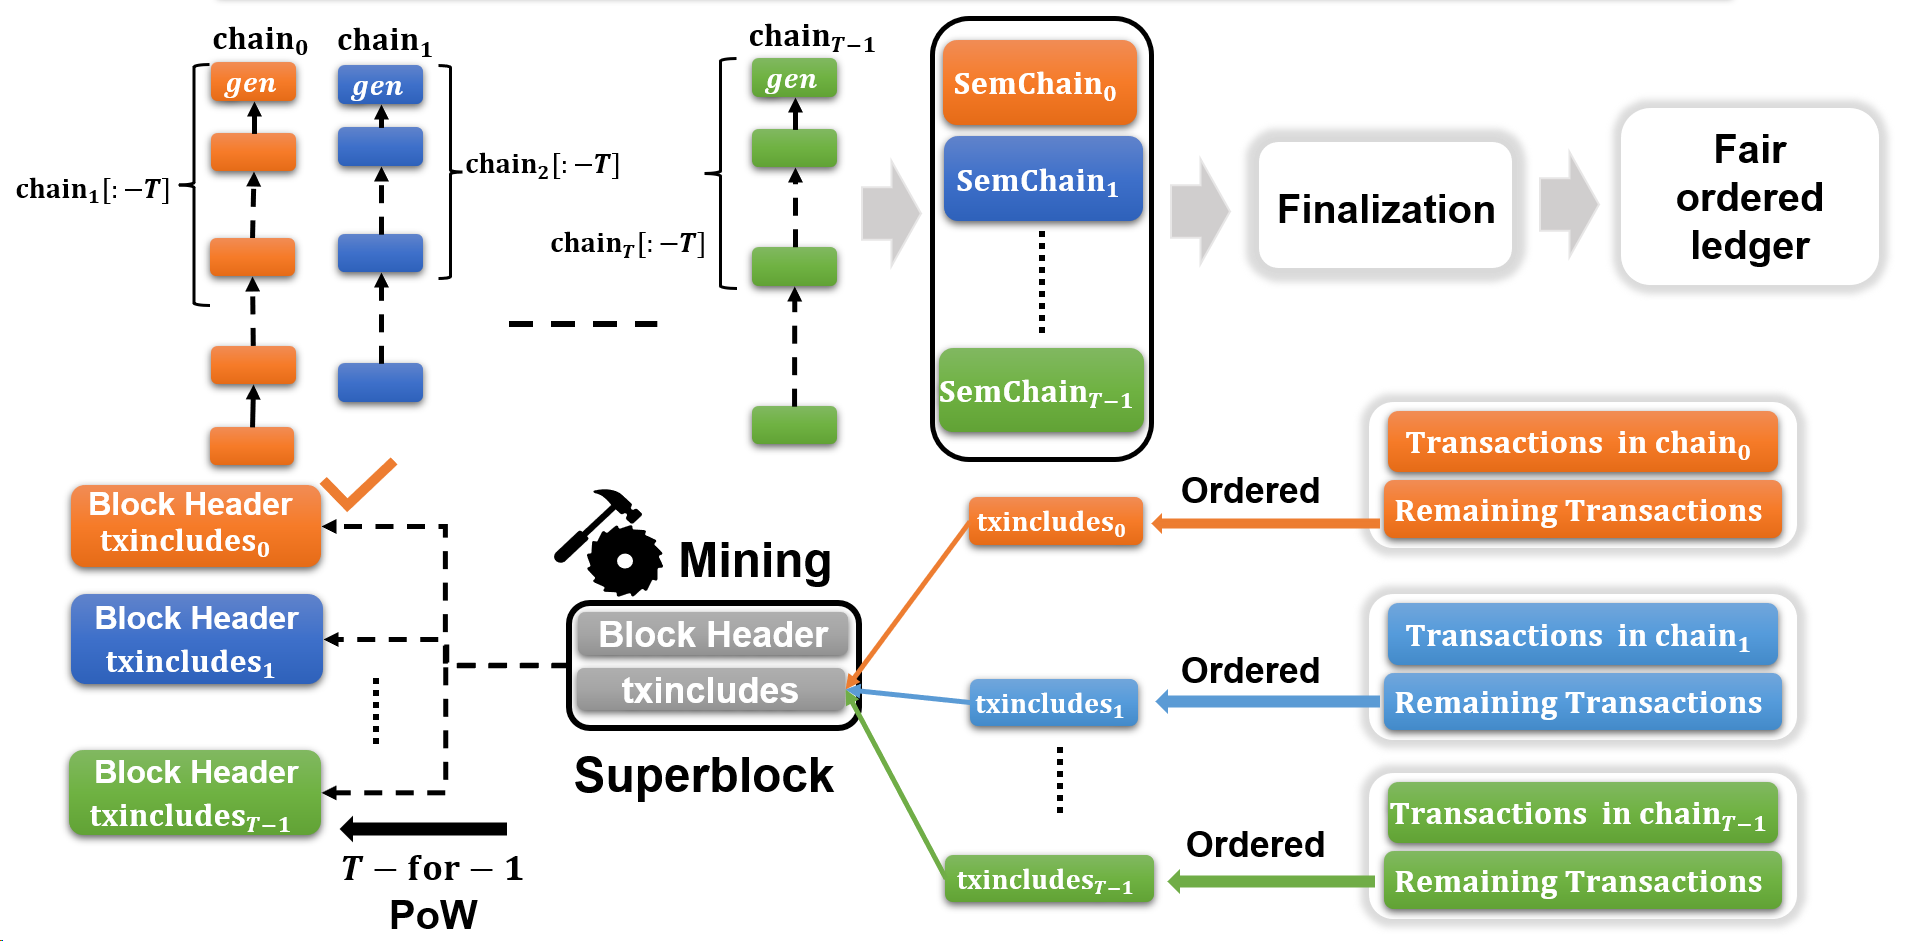
\includegraphics[width=0.85\linewidth]{Fig/21/F10}
	\caption{Multi chain}
	\label{fig:L21_f10}
\end{figure}
In a multi-chain system, mining is done by creating a superblock, which is a large block that contains many transactions. A superblock is mined by a group of nodes that cooperate and share the reward. A superblock can be mined faster than a single block, and can reduce the number of orphaned blocks. A multi-chain system can finalize transactions faster than a single chain system, and can tolerate more Byzantine faults.

\subsection{Zero-Block Confirmation}
Latency can affect the performance and security of a blockchain system, especially in scenarios where fast and reliable transactions are required. For example, Alice pays 0.0001 bitcoin to a coffee shop using her smartphone. However, the transaction takes too long to be confirmed by the network, and by the time it is confirmed, the coffee shop has already closed. This means that Alice has paid for a coffee that she cannot receive, and the coffee shop has lost a potential customer.
\begin{figure}[h!]
	\centering
	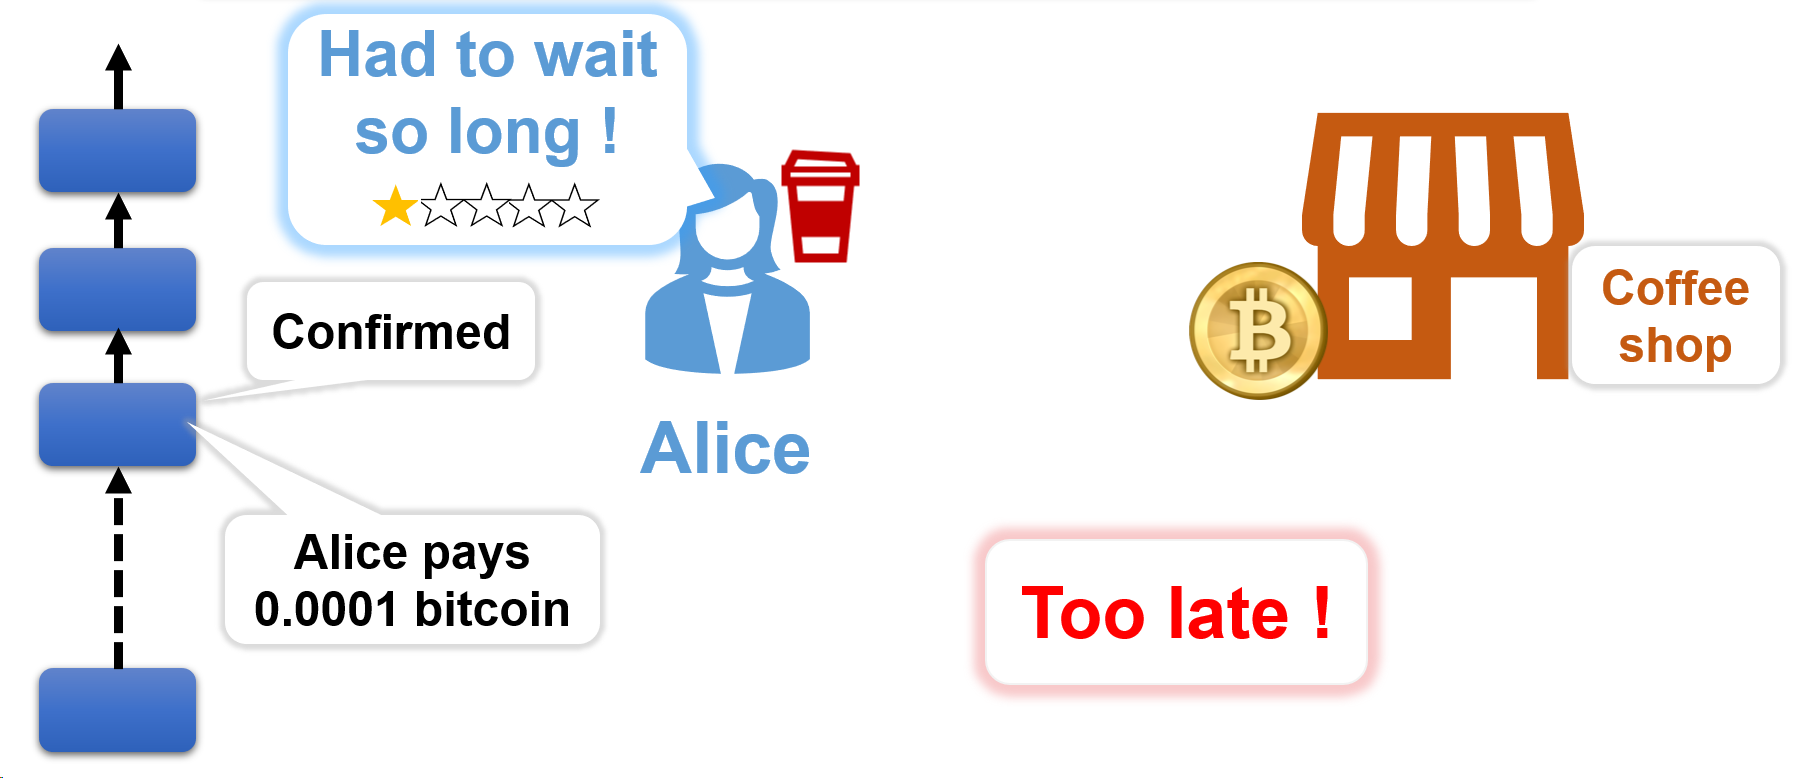
\includegraphics[width=0.7\linewidth]{Fig/21/F11}
	\caption{Latency matters!}
	\label{fig:L21_f11}
\end{figure}\\\\
One way to reduce latency in blockchain systems is to use zero-block confirmation, which is a technique that allows transactions to be accepted without waiting for them to be included in a block. Zero-block confirmation relies on the assumption that most nodes in the network are honest and will not try to double-spend or reverse transactions.\\\\
However, zero-block confirmation also has some drawbacks, such as being vulnerable to attacks such as 51\% attack, where a malicious node can control more than half of the network’s computing power and create a longer chain that invalidates previous transactions. Therefore, zero-block confirmation is not a secure or reliable solution for reducing latency in blockchain systems.
